\chapter{Resultados}\label{cap:resultados}

Este capítulo presenta los resultados de la corrida principal, con la partición sin el cierre
del mercado. Primero se muestra que esa partición recupera una prueba informativa (Sección
\ref{sec:res_cierre}) y cómo rinden los modelos según el escenario y la pérdida (Sección
\ref{sec:res_rend}). Después se contrastan las tres hipótesis (Secciones \ref{sec:res_h1} a
\ref{sec:res_h3}) y se examina qué parte de la estabilidad medida depende del modelo (Sección
\ref{sec:res_control}). Salvo que se indique otra cosa, cada cifra es la media de tres
semillas de modelo.

\section{La partición sin el cierre recupera la prueba}\label{sec:res_cierre}

La Figura \ref{fig:cierre} compara el rendimiento en prueba de las dos particiones, en el
escenario nativo y con la pérdida que obtuvo el mayor PR-AUC de validación para cada
arquitectura. Con la partición original, cuya prueba cae después del cierre, ningún modelo
supera al azar. Sin el cierre, tres de las cuatro arquitecturas detectan: GraphSAGE alcanza un
PR-AUC de 0,273, TAGCN de 0,244 y GAT de 0,172, entre 7 y 12 veces el valor del azar (0,023).
GCN queda en 0,085. El ROC-AUC sube de valores entre 0,48 y 0,71 a valores entre 0,73 y 0,88.
El mejor modelo de toda la matriz, GraphSAGE con pesos por clase en el escenario 1:20, obtiene
en prueba un PR-AUC de 0,306 y un ROC-AUC de 0,901.

\begin{figure}[ht]
\centering
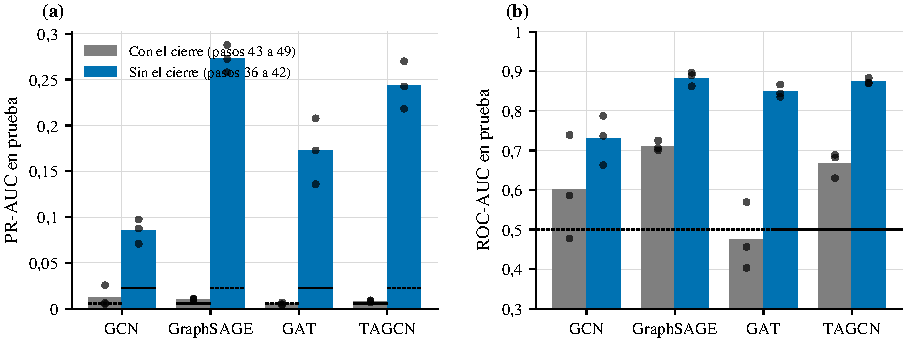
\includegraphics[width=\textwidth]{efecto_cierre}
\caption{Rendimiento en prueba con la partición original (prueba en los pasos 43 a 49,
después del cierre) y con la partición sin el cierre (prueba en los pasos 36 a 42). Escenario
nativo, pérdida elegida por validación. Las barras son la media de tres semillas, los puntos
cada semilla y las líneas discontinuas el valor del azar: la prevalencia en (a) y 0,5 en (b).}
\label{fig:cierre}
\end{figure}

La Figura \ref{fig:curvas_test} muestra las curvas completas. La curva de precisión y
exhaustividad deja ver lo que el ROC-AUC oculta: con la mitad de las ilícitas recuperadas, la precisión de GraphSAGE y de TAGCN
ronda 0,3, es decir, unas dos falsas alarmas por cada acierto. La Tabla \ref{tab:rend_nativo}
resume las cifras.

\begin{figure}[ht]
\centering
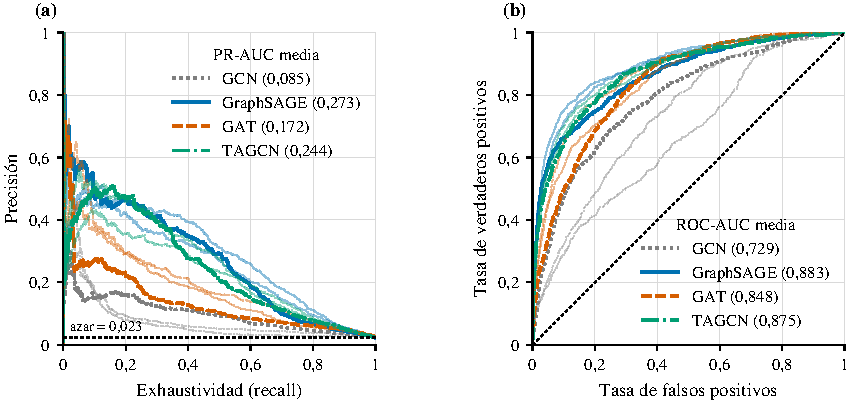
\includegraphics[width=\textwidth]{curvas_nativo_test}
\caption{Curvas de precisión y exhaustividad (a) y ROC (b) en la prueba de la partición sin el
cierre, escenario nativo, con la pérdida elegida por validación para cada arquitectura. Trazo
grueso: semilla 42; trazos finos: semillas 43 y 44. Entre paréntesis, el área media de las tres
semillas.}
\label{fig:curvas_test}
\end{figure}

\begin{table}[ht]
\centering
\caption{Rendimiento en el escenario nativo con la pérdida elegida por validación (media
$\pm$ desviación estándar de tres semillas). Filtro: modelos que superan el filtro de calidad
en validación.}
\label{tab:rend_nativo}
\small
% Generado por tesis_v4/scripts/analisis.py. No editar a mano.
\begin{tabular}{llcccc}
\toprule
Arquitectura & Pérdida elegida & PR-AUC val. & PR-AUC prueba & ROC-AUC prueba & Filtro \\
\midrule
GCN & Focal loss & 0{,}214 $\pm$ 0{,}054 & 0{,}085 $\pm$ 0{,}013 & 0{,}729 $\pm$ 0{,}063 & 0/3 \\
GraphSAGE & Focal loss & 0{,}478 $\pm$ 0{,}038 & 0{,}273 $\pm$ 0{,}015 & 0{,}883 $\pm$ 0{,}018 & 3/3 \\
GAT & Sin ajuste & 0{,}282 $\pm$ 0{,}027 & 0{,}172 $\pm$ 0{,}036 & 0{,}848 $\pm$ 0{,}016 & 2/3 \\
TAGCN & Focal loss & 0{,}529 $\pm$ 0{,}074 & 0{,}244 $\pm$ 0{,}026 & 0{,}875 $\pm$ 0{,}007 & 3/3 \\
\midrule
Azar & & 0{,}037 & 0{,}023 & 0{,}5 & \\
\bottomrule
\end{tabular}

\end{table}

\section{Rendimiento según el escenario y la pérdida}\label{sec:res_rend}

La Figura \ref{fig:perdida} y la Tabla \ref{tab:rend_esc} muestran el PR-AUC de validación de
cada combinación. Tres regularidades se observan.

\textbf{La mejor pérdida depende del escenario.} En el escenario nativo, \textit{focal loss}
iguala o supera a los pesos por clase: en GraphSAGE, 0,478 frente a 0,326; en TAGCN, 0,529
frente a 0,212. En 1:10, la entropía sin ajuste es la mejor en ambas (0,551 y 0,594). No hay
una pérdida que sea la mejor en todos los escenarios.

\textbf{Con poco fraude solo resisten los pesos por clase.} En 1:100 y 1:200, la
\textit{focal loss} de GraphSAGE cae a 0,189 y 0,054, y la de TAGCN a 0,282 y 0,054. Los pesos
por clase mantienen a GraphSAGE en 0,447 y 0,420, y a TAGCN en 0,357 y 0,307. Es el mismo
comportamiento que en la partición original.

\textbf{La entropía sin ajuste es frágil.} En GraphSAGE pasa de 0,551 en 1:10 a 0,035 en 1:20
y se queda en el nivel del azar en todos los escenarios más desbalanceados; en TAGCN baja de
0,594 a 0,046 entre 1:10 y 1:100. Cuando el desbalance supera cierto punto, el modelo minimiza
la pérdida prediciendo casi siempre la clase negativa. GAT es la excepción: es la arquitectura
en la que la entropía sin ajuste supera más veces el filtro de calidad (Tabla \ref{tab:filtro}).

\begin{figure}[ht]
\centering
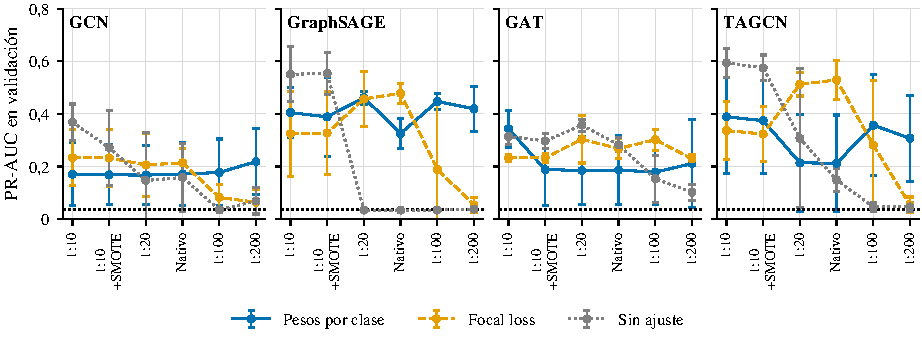
\includegraphics[width=\textwidth]{perdida_por_escenario}
\caption{PR-AUC de validación por escenario y pérdida (media y desviación estándar de tres
semillas). La línea discontinua es el valor del azar (0,037).}
\label{fig:perdida}
\end{figure}

\begin{table}[ht]
\centering
\caption{PR-AUC de validación por escenario, arquitectura y pérdida (media de tres semillas).}
\label{tab:rend_esc}
\scriptsize
\setlength{\tabcolsep}{4pt}
% Generado por tesis_v4/scripts/analisis.py. No editar a mano.
\begin{tabular}{llcccccc}
\toprule
Arquitectura & Pérdida & 1:10 & 1:10 + SMOTE & 1:20 & Nativo & 1:100 & 1:200 \\
\midrule
GCN & Pesos por clase & 0{,}171 & 0{,}169 & 0{,}167 & 0{,}171 & 0{,}177 & 0{,}219 \\
 & Focal loss & 0{,}234 & 0{,}233 & 0{,}206 & 0{,}214 & 0{,}083 & 0{,}064 \\
 & Sin ajuste & 0{,}369 & 0{,}271 & 0{,}147 & 0{,}159 & 0{,}035 & 0{,}069 \\
\midrule
GraphSAGE & Pesos por clase & 0{,}405 & 0{,}389 & 0{,}462 & 0{,}326 & 0{,}447 & 0{,}420 \\
 & Focal loss & 0{,}325 & 0{,}327 & 0{,}457 & 0{,}478 & 0{,}189 & 0{,}054 \\
 & Sin ajuste & 0{,}551 & 0{,}554 & 0{,}035 & 0{,}034 & 0{,}034 & 0{,}038 \\
\midrule
GAT & Pesos por clase & 0{,}344 & 0{,}188 & 0{,}185 & 0{,}187 & 0{,}179 & 0{,}211 \\
 & Focal loss & 0{,}233 & 0{,}233 & 0{,}304 & 0{,}268 & 0{,}302 & 0{,}229 \\
 & Sin ajuste & 0{,}314 & 0{,}297 & 0{,}357 & 0{,}282 & 0{,}154 & 0{,}102 \\
\midrule
TAGCN & Pesos por clase & 0{,}389 & 0{,}374 & 0{,}214 & 0{,}212 & 0{,}357 & 0{,}307 \\
 & Focal loss & 0{,}337 & 0{,}323 & 0{,}512 & 0{,}529 & 0{,}282 & 0{,}054 \\
 & Sin ajuste & 0{,}594 & 0{,}575 & 0{,}307 & 0{,}149 & 0{,}046 & 0{,}046 \\
\bottomrule
\end{tabular}

\end{table}

\textbf{GCN no aprende en este problema.} Ningún modelo GCN con pesos por clase supera el filtro
de calidad (Tabla \ref{tab:filtro}). GCN promedia a cada transacción con sus vecinas sin darle
un peso propio (Sección \ref{sec:gnn}), y en Elliptic la señal está sobre todo en la propia
transacción. Por eso los análisis de estabilidad por escenario y por pérdida se restringen a
GraphSAGE, GAT y TAGCN, y GCN se incluye solo en la comparación entre arquitecturas, con esa
salvedad. Hay que añadir que GAT con pesos por clase tampoco supera el filtro en ningún modelo,
aunque su PR-AUC de validación esté entre 0,18 y 0,34, muy por encima del azar: el filtro usa
el umbral fijo de 0,5, y con ese umbral su F1 queda entre 0,13 y 0,17. Se mantiene en el
análisis porque su PR-AUC muestra que sí ordena las transacciones mejor que el azar.

\begin{table}[ht]
\centering
\caption{Modelos que superan el filtro de calidad en validación (F1 $\geq$ 0,30 y MCC $\geq$
0,15 con umbral 0,5), de 18 por celda (6 escenarios por 3 semillas).}
\label{tab:filtro}
\small
% Generado por tesis_v4/scripts/analisis.py. No editar a mano.
\begin{tabular}{lccc}
\toprule
Arquitectura & Pesos por clase & Focal loss & Sin ajuste \\
\midrule
GCN & 0/18 & 3/18 & 6/18 \\
GraphSAGE & 10/18 & 11/18 & 6/18 \\
GAT & 0/18 & 8/18 & 11/18 \\
TAGCN & 8/18 & 13/18 & 7/18 \\
\bottomrule
\end{tabular}

\end{table}

\section{H1: el nivel de desbalance no cambia la estabilidad}\label{sec:res_h1}

La Figura \ref{fig:h1} y la Tabla \ref{tab:h1} muestran la estabilidad entre réplicas de cada
explicador en los seis escenarios, con pesos por clase y las tres arquitecturas que aprenden.
Con la medida principal, la estabilidad de GNNExplainer se mueve entre 0,917 (nativo) y 0,939
(1:100), la de Shapley entre 0,991 y 0,994 y la de Expected Gradients entre 0,918 y 0,934.
Integrated Gradients es determinista y vale 1 en todos los casos. No hay una tendencia a bajar
a medida que el desbalance se hace más extremo: 1:100 y 1:200 no son los escenarios menos
estables. Las dos medidas robustas confirman la ausencia de tendencia, aunque con valores más
bajos (Sección \ref{sec:res_control}).

\begin{figure}[ht]
\centering
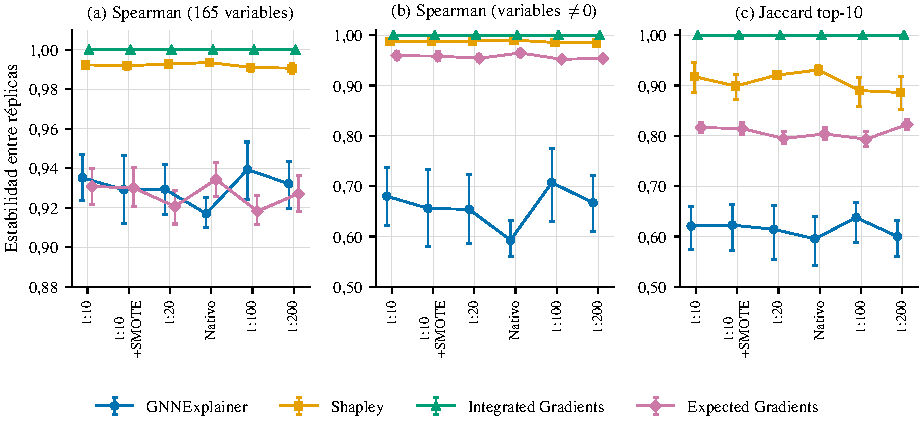
\includegraphics[width=\textwidth]{estabilidad_por_escenario}
\caption{Estabilidad entre réplicas por escenario y explicador, con las tres medidas. Pesos
por clase; media de 9 modelos (3 arquitecturas que aprenden por 3 semillas) e intervalo
\textit{bootstrap} del 95~\%.}
\label{fig:h1}
\end{figure}

\begin{table}[ht]
\centering
\caption{Estabilidad entre réplicas por escenario (pesos por clase, 9 modelos). $p$ Friedman:
igualdad de los seis escenarios. $p$ TOST: equivalencia entre nativo y 1:200 con margen 0,05
(un valor bajo indica equivalencia).}
\label{tab:h1}
\scriptsize
\setlength{\tabcolsep}{3.5pt}
% Generado por tesis_v4/scripts/analisis.py. No editar a mano.
\begin{tabular}{llcccccccc}
\toprule
Medida & Explicador & 1:10 & 1:10 + SMOTE & 1:20 & Nativo & 1:100 & 1:200 & $p$ Friedman & $p$ TOST \\
\midrule
Spearman global & GNNExplainer & 0{,}935 & 0{,}929 & 0{,}929 & 0{,}917 & 0{,}939 & 0{,}932 & 0{,}269 & $<0{,}001$ \\
 & Shapley & 0{,}992 & 0{,}992 & 0{,}993 & 0{,}994 & 0{,}991 & 0{,}991 & 0{,}534 & $<0{,}001$ \\
 & Integrated Gradients & 1{,}000 & 1{,}000 & 1{,}000 & 1{,}000 & 1{,}000 & 1{,}000 & -- & $<0{,}001$ \\
 & Expected Gradients & 0{,}931 & 0{,}930 & 0{,}921 & 0{,}934 & 0{,}918 & 0{,}927 & 0{,}248 & $<0{,}001$ \\
\midrule
Spearman $\neq 0$ & GNNExplainer & 0{,}680 & 0{,}656 & 0{,}654 & 0{,}593 & 0{,}707 & 0{,}667 & 0{,}117 & 0{,}791 \\
 & Shapley & 0{,}988 & 0{,}987 & 0{,}988 & 0{,}990 & 0{,}985 & 0{,}985 & 0{,}448 & $<0{,}001$ \\
 & Integrated Gradients & 1{,}000 & 1{,}000 & 1{,}000 & 1{,}000 & 1{,}000 & 1{,}000 & -- & $<0{,}001$ \\
 & Expected Gradients & 0{,}959 & 0{,}958 & 0{,}954 & 0{,}965 & 0{,}952 & 0{,}954 & 0{,}552 & $<0{,}001$ \\
\midrule
Jaccard top-10 & GNNExplainer & 0{,}621 & 0{,}623 & 0{,}614 & 0{,}595 & 0{,}638 & 0{,}600 & 0{,}233 & 0{,}012 \\
 & Shapley & 0{,}918 & 0{,}899 & 0{,}921 & 0{,}931 & 0{,}890 & 0{,}886 & 0{,}117 & 0{,}394 \\
 & Integrated Gradients & 1{,}000 & 1{,}000 & 1{,}000 & 1{,}000 & 1{,}000 & 1{,}000 & -- & $<0{,}001$ \\
 & Expected Gradients & 0{,}816 & 0{,}814 & 0{,}795 & 0{,}804 & 0{,}793 & 0{,}823 & 0{,}018 & $<0{,}001$ \\
\bottomrule
\end{tabular}

\end{table}

Las pruebas confirman la lectura visual. Con la medida principal, la prueba de Friedman no
rechaza la igualdad de los seis escenarios para ningún explicador ($p = 0{,}27$ en
GNNExplainer, $0{,}53$ en Shapley y $0{,}25$ en Expected Gradients), y la prueba de
equivalencia entre el nativo y 1:200 la acepta en los tres ($p \leq 0{,}0002$): la diferencia
entre el escenario real y el más extremo es menor que 0,05. Con las medidas robustas hay dos
excepciones que conviene examinar. Con el Jaccard top-10, Friedman rechaza la igualdad en
Expected Gradients ($p = 0{,}018$), pero la diferencia entre el mejor y el peor escenario es de
0,03 y el escenario más estable es precisamente 1:200; no hay degradación. Con el Spearman sobre
las variables distintas de cero, GNNExplainer no alcanza la equivalencia ($p = 0{,}79$): sus
valores van de 0,593 (nativo) a 0,707 (1:100), con un intervalo amplio, pero de nuevo el
escenario menos estable es el nativo y no los más desbalanceados.

\textbf{Veredicto sobre H1.} La hipótesis no se sostiene. En ninguno de los cuatro explicadores
ni con ninguna de las tres medidas la estabilidad disminuye a medida que el desbalance se hace
más extremo, ni siquiera en 1:100 y 1:200, donde además se quitaron transacciones ilícitas del
entrenamiento. El mismo resultado se obtuvo con la partición original (Anexo
\ref{anx:original}).

\section{H2: no hay un orden estable entre arquitecturas}\label{sec:res_h2}

\begin{figure}[ht]
\centering
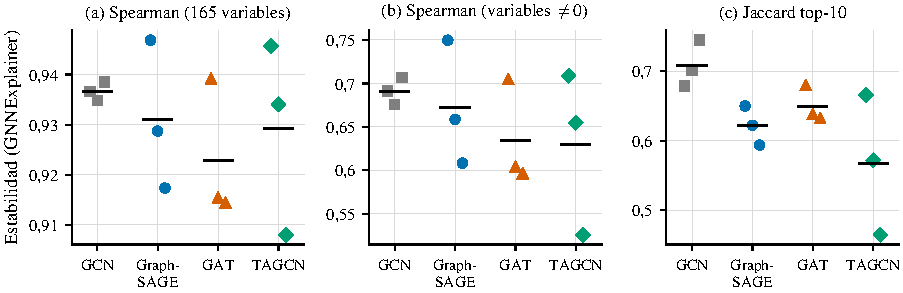
\includegraphics[width=\textwidth]{estabilidad_por_arquitectura}
\caption{Estabilidad de GNNExplainer por arquitectura con las tres medidas (pesos por clase,
media de los cuatro escenarios principales). Cada punto es una semilla; la línea horizontal es
la media.}
\label{fig:h2}
\end{figure}

\begin{table}[ht]
\centering
\caption{Estabilidad por arquitectura (pesos por clase, media de los escenarios principales,
3 semillas). $p$ (4): Friedman con las cuatro arquitecturas; $p$ (3): sin GCN. Primera: número
de semillas en que cada arquitectura obtiene el mayor valor.}
\label{tab:h2}
\scriptsize
\setlength{\tabcolsep}{3.5pt}
% Generado por tesis_v4/scripts/analisis.py. No editar a mano.
\begin{tabular}{llccccccl}
\toprule
Medida & Explicador & GCN & GraphSAGE & GAT & TAGCN & $p$ (4) & $p$ (3) & Primera \\
\midrule
Spearman global & GNNExplainer & 0{,}937 & 0{,}931 & 0{,}923 & 0{,}929 & 0{,}532 & 0{,}264 & GCN 2, GraphSAGE 1 \\
 & Shapley & 0{,}996 & 0{,}994 & 0{,}994 & 0{,}991 & 0{,}042 & 0{,}097 & GCN 3 \\
 & Expected Gradients & 0{,}923 & 0{,}935 & 0{,}932 & 0{,}920 & 0{,}172 & 0{,}097 & GraphSAGE 2, GAT 1 \\
\midrule
Spearman $\neq 0$ & GNNExplainer & 0{,}691 & 0{,}672 & 0{,}635 & 0{,}630 & 0{,}334 & 0{,}097 & GCN 2, GraphSAGE 1 \\
 & Shapley & 0{,}993 & 0{,}991 & 0{,}990 & 0{,}985 & 0{,}042 & 0{,}097 & GCN 3 \\
 & Expected Gradients & 0{,}958 & 0{,}965 & 0{,}960 & 0{,}952 & 0{,}457 & 0{,}264 & GAT 1, GraphSAGE 1, GCN 1 \\
\midrule
Jaccard top-10 & GNNExplainer & 0{,}708 & 0{,}622 & 0{,}650 & 0{,}568 & 0{,}060 & 0{,}097 & GCN 2, GAT 1 \\
 & Shapley & 0{,}948 & 0{,}929 & 0{,}927 & 0{,}896 & 0{,}122 & 0{,}264 & GCN 2, GraphSAGE 1 \\
 & Expected Gradients & 0{,}798 & 0{,}800 & 0{,}816 & 0{,}806 & 0{,}532 & 0{,}264 & GAT 2, GCN 1 \\
\bottomrule
\end{tabular}

\end{table}

Con GNNExplainer, las cuatro arquitecturas quedan dentro de dos centésimas con la medida
principal (de 0,923 en GAT a 0,937 en GCN), y las semillas de una misma arquitectura se
dispersan tanto como las arquitecturas entre sí (Figura \ref{fig:h2}). Ninguna prueba de
Friedman rechaza la igualdad con GNNExplainer ($p$ entre 0,06 y 0,53) ni con Expected
Gradients, y sin GCN ninguna lo hace con ningún explicador ni medida ($p \geq 0{,}097$). La
única diferencia significativa aparece con Shapley y las cuatro arquitecturas ($p = 0{,}042$):
GCN es la más estable en las tres semillas, pero la diferencia con la última es de cinco
milésimas (0,996 frente a 0,991). Con tres semillas como bloques la prueba tiene poca potencia,
por lo que la ausencia de diferencias no prueba la igualdad; lo que sí muestra es que no hay un
orden que se repita.

Un resultado llama la atención: GCN, la arquitectura que no aprende, obtiene las explicaciones
más estables con GNNExplainer en dos de las tres semillas y en las tres medidas. Esto anticipa
lo que muestra la Sección \ref{sec:res_control}: una explicación estable no es necesariamente
una explicación de algo aprendido.

\textbf{Veredicto sobre H2.} La hipótesis no se sostiene entre las arquitecturas que aprenden:
GraphSAGE, GAT y TAGCN producen explicaciones con estabilidad indistinguible. En la partición
original GraphSAGE había resultado la más estable en las tres semillas; ese orden no se repite
sin el cierre, y por tanto no se puede afirmar.

\section{H3: la técnica de compensación no cambia la estabilidad}\label{sec:res_h3}

\begin{table}[ht]
\centering
\caption{Estabilidad por técnica de compensación (3 arquitecturas que aprenden, media de los
escenarios principales). PC $>$ FL y PC $>$ SA: en cuántos de los 9 pares de arquitectura y
semilla pesos por clase supera a \textit{focal loss} o a sin ajuste, con el $p$ de la prueba
de signos.}
\label{tab:h3}
\scriptsize
\setlength{\tabcolsep}{3.5pt}
% Generado por tesis_v4/scripts/analisis.py. No editar a mano.
\begin{tabular}{llccccc}
\toprule
Medida & Explicador & Pesos por clase & Focal loss & Sin ajuste & PC $>$ FL & PC $>$ SA \\
\midrule
Spearman global & GNNExplainer & 0{,}928 & 0{,}922 & 0{,}930 & 6.0/9 (0{,}508) & 4.0/9 (1{,}000) \\
 & Shapley & 0{,}993 & 0{,}995 & 0{,}994 & 0.0/9 (0{,}004) & 5.0/9 (1{,}000) \\
 & Expected Gradients & 0{,}929 & 0{,}933 & 0{,}938 & 2.0/9 (0{,}180) & 1.0/9 (0{,}039) \\
\midrule
Spearman $\neq 0$ & GNNExplainer & 0{,}646 & 0{,}626 & 0{,}668 & 5.0/9 (1{,}000) & 2.0/9 (0{,}180) \\
 & Shapley & 0{,}988 & 0{,}992 & 0{,}990 & 1.0/9 (0{,}039) & 4.0/9 (1{,}000) \\
 & Expected Gradients & 0{,}959 & 0{,}960 & 0{,}962 & 4.0/9 (1{,}000) & 4.0/9 (1{,}000) \\
\midrule
Jaccard top-10 & GNNExplainer & 0{,}613 & 0{,}598 & 0{,}625 & 5.0/9 (1{,}000) & 5.0/9 (1{,}000) \\
 & Shapley & 0{,}917 & 0{,}941 & 0{,}922 & 2.0/9 (0{,}180) & 5.0/9 (1{,}000) \\
 & Expected Gradients & 0{,}807 & 0{,}799 & 0{,}805 & 7.0/9 (0{,}180) & 4.0/9 (1{,}000) \\
\bottomrule
\end{tabular}

\end{table}

Con GNNExplainer, ninguna comparación es significativa con ninguna medida: pesos por clase
supera a \textit{focal loss} en 6 de los 9 pares con la medida principal ($p = 0{,}51$) y a
la entropía sin ajuste en 4 ($p = 1$), y las diferencias medias son menores que 0,025 con las
tres medidas. Con Shapley y Expected Gradients aparecen diferencias sistemáticas pero
minúsculas: con Shapley, \textit{focal loss} es más estable que pesos por clase en los 9 pares
($p = 0{,}004$), por dos milésimas; con Expected Gradients, la entropía sin ajuste supera a
pesos por clase en 8 de 9 ($p = 0{,}039$), por nueve milésimas. El sentido de la diferencia
cambia según el explicador, y en la corrida original con GNNExplainer era el contrario (Anexo
\ref{anx:original}).

\textbf{Veredicto sobre H3.} La hipótesis se sostiene en términos prácticos: la técnica de
compensación cambia mucho el rendimiento (Sección \ref{sec:res_rend}) pero mueve la estabilidad
de los explicadores de variables en milésimas o pocas centésimas, sin un sentido constante.

\begin{table}[ht]
\centering
\caption{Estabilidad de PGExplainer sobre las aristas del subgrafo: Spearman entre réplicas y
Jaccard de las 20 aristas principales (escenarios principales, media de 3 semillas).}
\label{tab:pg}
\small
% Generado por tesis_v4/scripts/analisis.py. No editar a mano.
\begin{tabular}{lcccccc}
\toprule
 & \multicolumn{2}{c}{Pesos por clase} & \multicolumn{2}{c}{Focal loss} & \multicolumn{2}{c}{Sin ajuste} \\
\cmidrule(lr){2-3}\cmidrule(lr){4-5}\cmidrule(lr){6-7}
Arquitectura & Spearman & Jaccard & Spearman & Jaccard & Spearman & Jaccard \\
\midrule
GCN & 0{,}517 & 0{,}630 & 0{,}325 & 0{,}645 & 0{,}322 & 0{,}608 \\
GraphSAGE & 0{,}251 & 0{,}560 & 0{,}064 & 0{,}628 & 0{,}381 & 0{,}658 \\
GAT & 0{,}305 & 0{,}621 & 0{,}514 & 0{,}625 & 0{,}458 & 0{,}675 \\
TAGCN & 0{,}504 & 0{,}769 & 0{,}121 & 0{,}628 & 0{,}288 & 0{,}650 \\
\bottomrule
\end{tabular}

\end{table}

\textbf{PGExplainer.} PGExplainer explica aristas y no variables, por lo que se analiza aparte
(Tabla \ref{tab:pg}). El grafo de Elliptic es muy disperso: la mediana de aristas en el
subgrafo receptivo de las transacciones explicadas es de 2 o 3, y la estabilidad solo se pudo
medir, en promedio, en 13 de las 30 transacciones (las demás tienen menos aristas de las
necesarias para comparar órdenes). Con tan pocas aristas, el Spearman entre réplicas es una
medida muy gruesa y el Jaccard de las 20 principales compara casi siempre conjuntos que
incluyen todas las aristas disponibles. Aun así, el Spearman va de 0,06 a 0,52 según la
combinación, sin patrón por arquitectura ni por pérdida. La conclusión es que, en este
problema, PGExplainer no produce una explicación de aristas evaluable, y que la variación entre
pérdidas no puede atribuirse a la técnica de compensación.

\section{Qué parte de la estabilidad depende del modelo}\label{sec:res_control}

Las secciones anteriores muestran que la estabilidad apenas cambia con el escenario, la
arquitectura o la pérdida. Hay dos explicaciones posibles: que los modelos aprendan casi lo
mismo en todas las condiciones, o que la estabilidad medida no dependa de lo aprendido. El
control de pesos aleatorios (Sección \ref{sec:control}) permite distinguirlas (Figura
\ref{fig:control} y Tabla \ref{tab:control}).

\begin{figure}[ht]
\centering
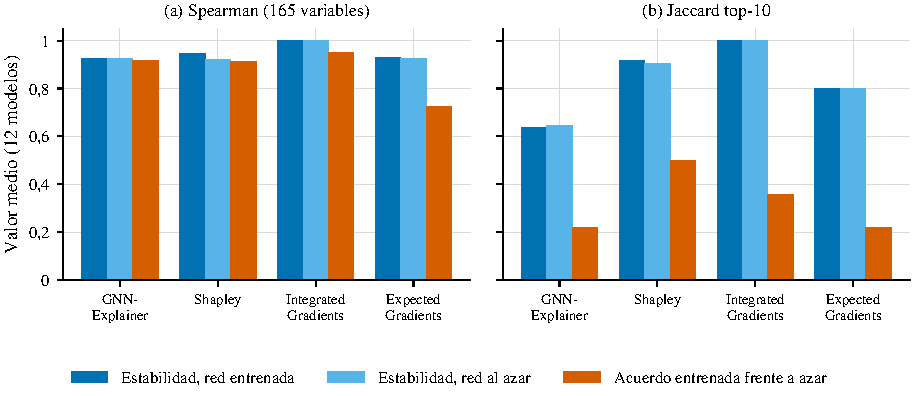
\includegraphics[width=\textwidth]{control_pesos_azar}
\caption{Control de pesos aleatorios en el escenario nativo con pesos por clase (12 modelos:
4 arquitecturas por 3 semillas). Para cada explicador, la estabilidad entre réplicas con la red
entrenada y con una red de pesos aleatorios, y el acuerdo entre la explicación de la red
entrenada y la de la red aleatoria.}
\label{fig:control}
\end{figure}

\begin{table}[ht]
\centering
\caption{Control de pesos aleatorios (media de 12 modelos).}
\label{tab:control}
\scriptsize
\setlength{\tabcolsep}{4pt}
% Generado por tesis_v4/scripts/analisis.py. No editar a mano.
\begin{tabular}{lcccccc}
\toprule
 & \multicolumn{3}{c}{Spearman global} & \multicolumn{3}{c}{Jaccard top-10} \\
\cmidrule(lr){2-4}\cmidrule(lr){5-7}
Explicador & Estab. entrenada & Estab. azar & Entrenada vs azar & Estab. entrenada & Estab. azar & Entrenada vs azar \\
\midrule
GNNExplainer & 0{,}924 & 0{,}927 & 0{,}917 & 0{,}636 & 0{,}646 & 0{,}220 \\
Shapley & 0{,}948 & 0{,}920 & 0{,}914 & 0{,}915 & 0{,}904 & 0{,}498 \\
Integrated Gradients & 1{,}000 & 1{,}000 & 0{,}950 & 1{,}000 & 1{,}000 & 0{,}357 \\
Expected Gradients & 0{,}932 & 0{,}924 & 0{,}724 & 0{,}801 & 0{,}799 & 0{,}220 \\
\bottomrule
\end{tabular}

\end{table}

\textbf{Con la medida principal, la explicación no depende del modelo.} La explicación de
GNNExplainer sobre el modelo entrenado coincide con la de una red sin entrenar con un Spearman
de 0,917, prácticamente lo mismo que coinciden dos réplicas sobre el mismo modelo (0,924). Lo
mismo ocurre con Shapley (0,914 frente a 0,948) e Integrated Gradients (0,950). Una red con
pesos aleatorios, que no aprendió nada, recibe además explicaciones igual de estables que la
entrenada (0,927 en GNNExplainer). El orden de Integrated Gradients coincide con el orden de
las variables por su valor absoluto con un Spearman de 0,97. La medida principal está dominada
por el bloque de variables en cero (Sección \ref{sec:medidas}), que ocupa las mismas posiciones
del orden con cualquier red.

\textbf{Con el Jaccard top-10, sí depende.} Las 10 variables principales de la red entrenada y
de la aleatoria comparten en promedio un índice de 0,22 con GNNExplainer y Expected Gradients,
0,36 con Integrated Gradients y 0,50 con Shapley, muy por debajo de la estabilidad entre
réplicas (0,64, 0,80, 1 y 0,92). Las variables que el analista vería primero sí cambian con los
pesos del modelo. Expected Gradients es el único explicador cuyo acuerdo con la red aleatoria
también es claramente menor que su estabilidad con la medida principal (0,724 frente a 0,932),
porque sus referencias no son el vector cero y su atribución no se anula en las variables nulas.

\textbf{Modelos igual de buenos dan explicaciones distintas.} El acuerdo entre explicaciones de
modelos distintos refuerza esta lectura. Con GNNExplainer y pesos por clase, dos semillas de la
misma arquitectura y el mismo escenario coinciden con un Spearman global de 0,929, pero con un
Jaccard top-10 de solo 0,30: comparten unas 5 de sus 10 variables principales. Cambiar de
escenario manteniendo la semilla mueve menos la explicación (Jaccard 0,60) que cambiar de
semilla manteniendo el escenario. La principal fuente de variación de la explicación no es el
desbalance, sino la aleatoriedad del entrenamiento.

\textbf{Los explicadores no coinciden entre sí.} Sobre el mismo modelo, los cuatro explicadores
de variables señalan conjuntos de variables principales muy distintos (Figura
\ref{fig:explicadores}): con el Jaccard top-10 el acuerdo va de 0,10 (GNNExplainer frente a
Shapley) a 0,49 (Integrated frente a Expected Gradients). El alto Spearman global entre
GNNExplainer e Integrated Gradients (0,84) desaparece con el Jaccard top-10 (0,29), lo que
indica que su parecido se debe sobre todo al bloque de variables nulas.

\begin{figure}[ht]
\centering
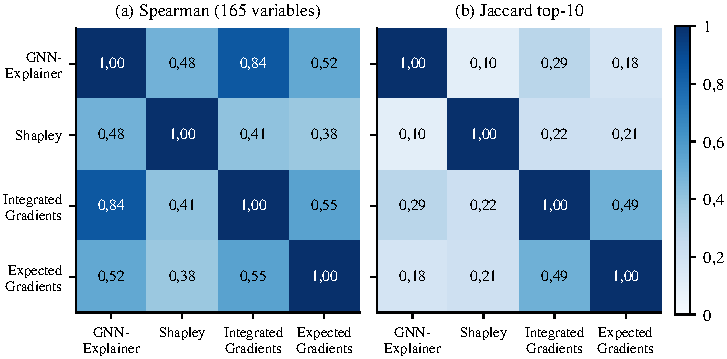
\includegraphics[width=\textwidth]{acuerdo_explicadores}
\caption{Acuerdo entre explicadores sobre el mismo modelo (GraphSAGE, GAT y TAGCN; escenarios
principales; todas las pérdidas y semillas), con el Spearman global (a) y el Jaccard top-10 (b).}
\label{fig:explicadores}
\end{figure}

\section{Síntesis}\label{sec:res_sintesis}

La Tabla \ref{tab:veredictos} resume el contraste de las hipótesis.

\begin{table}[ht]
\centering
\caption{Veredicto de las hipótesis con la partición sin el cierre.}
\label{tab:veredictos}
\small
\begin{tabularx}{\textwidth}{p{0.3\textwidth}Xp{0.2\textwidth}}
\toprule
Hipótesis & Resultado & Veredicto \\
\midrule
H1: la estabilidad baja con el desbalance & Sin tendencia en 4 explicadores y 3 medidas;
equivalencia entre nativo y 1:200 con la medida principal & No se sostiene \\
H2: la estabilidad depende de la arquitectura & Sin orden repetido entre GraphSAGE, GAT y
TAGCN; GCN, que no aprende, es la más estable & No se sostiene \\
H3: la compensación no cambia la estabilidad & Diferencias de milésimas o pocas centésimas,
con sentido que cambia según el explicador & Se sostiene en términos prácticos \\
\bottomrule
\end{tabularx}
\end{table}

Los tres veredictos tienen una lectura común que el control de pesos aleatorios aclara: con la
medida principal, la estabilidad refleja sobre todo la estructura de los datos de entrada y el
explicador, no lo que el modelo aprendió, y por eso apenas responde a los factores del diseño.
Las 10 variables principales, en cambio, sí dependen del modelo, y varían más entre semillas
que entre escenarios.
